% THIS DOCUMENT IS TAILORED TO REQUIREMENTS FOR SCIENTIFIC COMPUTING.  IT SHOULDN'T
% BE USED FOR NON-SCIENTIFIC COMPUTING PROJECTS
\documentclass[12pt]{article}

\usepackage{amsmath, mathtools}
\usepackage{amsfonts}
\usepackage{amssymb}
\usepackage{graphicx}
\usepackage{colortbl}
\usepackage{xr}
\usepackage{hyperref}
\usepackage{longtable}
\usepackage{xfrac}
\usepackage{tabularx}
\usepackage{float}
\usepackage{siunitx}
\usepackage{booktabs}
\usepackage{caption}
\usepackage{pdflscape}
\usepackage{afterpage}

\usepackage[round]{natbib}

%\usepackage{refcheck}

\hypersetup{
    bookmarks=true,         % show bookmarks bar?
      colorlinks=true,       % false: boxed links; true: colored links
    linkcolor=red,          % color of internal links (change box color with linkbordercolor)
    citecolor=green,        % color of links to bibliography
    filecolor=magenta,      % color of file links
    urlcolor=cyan           % color of external links
}

%% Comments

\usepackage{color}

\newif\ifcomments\commentstrue

\ifcomments
\newcommand{\authornote}[3]{\textcolor{#1}{[#3 ---#2]}}
\newcommand{\todo}[1]{\textcolor{red}{[TODO: #1]}}
\else
\newcommand{\authornote}[3]{}
\newcommand{\todo}[1]{}
\fi

\newcommand{\wss}[1]{\authornote{blue}{SS}{#1}} 
\newcommand{\plt}[1]{\authornote{magenta}{TPLT}{#1}} %For explanation of the template
\newcommand{\an}[1]{\authornote{cyan}{Author}{#1}}

%% Common Parts

\newcommand{\progname}{Minimization Analysis} % PUT YOUR PROGRAM NAME HERE
\newcommand{\authname}{%Team \#, Team Name
%\\ Student 1 name
%\\ Student 2 name
%\\ Student 3 name
\\ Ning Wang} % AUTHOR NAMES                  

\usepackage{hyperref}
    \hypersetup{colorlinks=true, linkcolor=blue, citecolor=blue, filecolor=blue,
                urlcolor=blue, unicode=false}
    \urlstyle{same}
                                


% For easy change of table widths
\newcommand{\colZwidth}{1.0\textwidth}
\newcommand{\colAwidth}{0.13\textwidth}
\newcommand{\colBwidth}{0.82\textwidth}
\newcommand{\colCwidth}{0.1\textwidth}
\newcommand{\colDwidth}{0.05\textwidth}
\newcommand{\colEwidth}{0.8\textwidth}
\newcommand{\colFwidth}{0.17\textwidth}
\newcommand{\colGwidth}{0.5\textwidth}
\newcommand{\colHwidth}{0.28\textwidth}

% Used so that cross-references have a meaningful prefix
\newcounter{defnum} %Definition Number
\newcommand{\dthedefnum}{GD\thedefnum}
\newcommand{\dref}[1]{GD\ref{#1}}
\newcounter{datadefnum} %Datadefinition Number
\newcommand{\ddthedatadefnum}{DD\thedatadefnum}
\newcommand{\ddref}[1]{DD\ref{#1}}
\newcounter{theorynum} %Theory Number
\newcommand{\tthetheorynum}{T\thetheorynum}
\newcommand{\tref}[1]{T\ref{#1}}
\newcounter{tablenum} %Table Number
\newcommand{\tbthetablenum}{T\thetablenum}
\newcommand{\tbref}[1]{TB\ref{#1}}
\newcounter{assumpnum} %Assumption Number
\newcommand{\atheassumpnum}{P\theassumpnum}
\newcommand{\aref}[1]{A\ref{#1}}
\newcounter{goalnum} %Goal Number
\newcommand{\gthegoalnum}{P\thegoalnum}
\newcommand{\gsref}[1]{GS\ref{#1}}
\newcounter{instnum} %Instance Number
\newcommand{\itheinstnum}{IM\theinstnum}
\newcommand{\iref}[1]{IM\ref{#1}}
\newcounter{reqnum} %Requirement Number
\newcommand{\rthereqnum}{P\thereqnum}
\newcommand{\rref}[1]{R\ref{#1}}
\newcounter{nfrnum} %NFR Number
\newcommand{\rthenfrnum}{NFR\thenfrnum}
\newcommand{\nfrref}[1]{NFR\ref{#1}}
\newcounter{lcnum} %Likely change number
\newcommand{\lthelcnum}{LC\thelcnum}
\newcommand{\lcref}[1]{LC\ref{#1}}

\usepackage{fullpage}

\newcommand{\deftheory}[9][Not Applicable]
{
\newpage
\noindent \rule{\textwidth}{0.5mm}

\paragraph{RefName: } \textbf{#2} \phantomsection 
\label{#2}

\paragraph{Label:} #3

\noindent \rule{\textwidth}{0.5mm}

\paragraph{Equation:}

#4

\paragraph{Description:}

#5

\paragraph{Notes:}

#6

\paragraph{Source:}

#7

\paragraph{Ref.\ By:}

#8

\paragraph{Preconditions for \hyperref[#2]{#2}:}
\label{#2_precond}

#9

\paragraph{Derivation for \hyperref[#2]{#2}:}
\label{#2_deriv}

#1

\noindent \rule{\textwidth}{0.5mm}

}

\begin{document}

\title{Software Requirements Specification for \progname
} 
\author{\authname}
\date{\today}
	
\maketitle

~\newpage

\pagenumbering{roman}

\tableofcontents

~\newpage

\section*{Revision History}

\begin{tabularx}{\textwidth}{p{3cm}p{2cm}X}
\toprule {\bf Date} & {\bf Version} & {\bf Notes}\\
\midrule
February 8th & 1.0 & Initial Release\\
\today & 2.0 & Second Release\\
\bottomrule
\end{tabularx}

~\newpage

\section{Reference Material}

This section records information for easy reference.

\subsection{Table of Units}

Throughout this document SI (Syst\`{e}me International d'Unit\'{e}s) is employed
as the unit system.  In addition to the basic units, several derived units are
used as described below.  For each unit, the symbol is given followed by a
description of the unit and the SI name.
~\newline

\renewcommand{\arraystretch}{1.2}
%\begin{table}[ht]
  \noindent \begin{tabular}{l l l} 
    \toprule		
    \textbf{symbol} & \textbf{unit} & \textbf{SI}\\
    \midrule 
    \si{\metre} & length & metre\\
    \si{\kWh} & energy	& kilowatt\\
    \si{\m^3} & volume	& cubic meter\\
    \si{\second} & time & second\\
    \si{\celsius} & temperature & centigrade\\
    \si{HM/s} & computational power & hashrate\\
    \si{\watt} & power & watt (W = \si{\joule\per\second})\\
    \bottomrule
  \end{tabular}
  %	\caption{Provide a caption}
%\end{table}

\bigskip
Additionally, currency for the total cost, is labelled by unit "CAD" which define Canadian dollars.
\\
%{The symbol for units named after people use capital letters, but the name of the unit itself uses lower case.  For instance, pascals use the symbol Pa, watts use the symbol W, teslas use the symbol T, newtons use the symbol N, etc.  The one exception to this is degree Celsius.  Details on writing metric units can be found on the 
 % \href{https://www.nist.gov/pml/weights-and-measures/writing-metric-units}
 % {NIST} web-page.}

\subsection{Table of Symbols}

The table that follows summarizes the symbols used in this document along with their units. The choice of symbols was made to be consistent with existing documentation for electricity distribution systems.  The symbols are listed in alphabetical order.

\renewcommand{\arraystretch}{1.2}
%\noindent \begin{tabularx}{1.0\textwidth}{l l X}
\noindent \begin{longtable*}{l l p{12cm}} \toprule
\textbf{symbol} & \textbf{unit} & \textbf{description}\\
\midrule 

$L_\text{total}$ & \si[per-mode=symbol] {\watt} &total power demanded by the given combination plan
\\ 
$R_\text{total}$ & \si[per-mode=symbol] {\watt} &total electricity supply by the renewable energy\\
$P_\text{total}$ & \si[per-mode=symbol] {\watt} &total electricity supply by the distributed energy\\
\bottomrule
\end{longtable*}
%{Use your problems actual symbols.  The si package is a good idea to use for units.}

\subsection{Abbreviations and Acronyms}

\renewcommand{\arraystretch}{1.2}
\begin{tabular}{l l} 
  \toprule		
  \textbf{symbol} & \textbf{description}\\
  \midrule 
 $C_\text{total}$ & total cost\\
  $C_r$ & renewable cost\\
  $C_p$ & grid electricity cost\\
  $d_i$ & Distance between data center and power station\\
  $A_i$ & Computational power for data center\\
  IM & Instance Model\\
  LC & Likely Change\\
  PS & Physical System Description\\
  R & Requirement\\
  SRS & Software Requirements Specification\\
%  \progname{} & {put an expanded version of your program name here (as appropriate)}\\

  \bottomrule
\end{tabular}\\

%{Add any other abbreviations or acronyms that you add}

%\subsection{Mathematical Notation}

%{This section is optional but should be included for projects that make use of notation to convey mathematical information.  For instance, if typographic}
 

%{This section was added to the template because some students use very.}


\newpage
\section{Introduction}
Data centers use about 1\%-4\% of the electricity in the world\textsuperscript{\cite{rivier2013electricity}}. Using energy more efficiently is one of the fastest, most cost-effective ways to save money, reduce greenhouse gas emissions, create jobs, and meet growing energy demand. This project aims to minimize the total energy cost for a set of data centers by determining the optimal power consumption from renewable energy sources and the power grid.To get started, please provide a CSV file containing information about the data centers, such as their distances to renewable energy sources and their maximum power consumption. You will also be asked to input any restrictions on the Grid Power and Renewable Power limits.
The program will then process the input data, set up an optimization problem, and solve it using a linear programming approach. The resulting optimal power consumption for each data center will be displayed, along with the total cost of the energy. A plot illustrating the relationship between the distances to data centers and their optimal power consumption will also be provided for further analysis.

\subsection{Purpose of Document}

{The purpose of this document is to provide a analytical model of allocate the computing power to each data center with minimize the cost to program users (Section~\ref{sec_assumpt}).  This document should clearly
communicate all necessary background information and detailed system context is described in Section 3.}

\subsection{Scope of Requirements} 

 {The domain of this problem is restricted to given renewable energy pricing and factory electricity loss proportionate to transmission. In particular, different areas will have varying electricity pricing and distinct types of renewable resources. However, we can set constant renewable pricing and minimize the total cost to determine the optimal computing distribution plan for each data center. The domain focuses on one specific type of input data: the distance between the data center and the power station. In this program, specifically, we will identify the optimal cases of combination under static pricing. Therefore, it has been decided to use distances as input. Subsequently, since this project is limited to any renewable energy with a given price, any transmission power loss of renewable energy is considered out of scope. Essentially, while this program is intended to eventually be used within the context of specific physical data, it is developed and constructed for application to another area in North America as well.}  

%{The scope section is related to the assumptions section(Section~\ref{sec_assumpt}).  However, the scope and the assumptions are not at the same level of abstraction.  The scope is at a high level.  The focus is on the ``big picture'' assumptions.  The assumptions section lists, and describes, all of the assumptions.}

\subsection{Characteristics of Intended Reader} \label{sec_IntendedReader}

{This document assumes the intended reader has familiarity with basic optimization analysis, power system analysis, and electricity distribution analysis. Courses which contribute to background knowledge may be titled Linear Systems (undergrad), Electric Machines and Power Systems (undergrad), Electric Power Transmission, Distribution and Utilization (undergrad). Data constrain and model limitation will be discussed in this document. However, our exposition will only cover the concepts needed for our purposes. For proofs and for a complete exposition of all background materials. Furthermore, this document will explain as entry as possible aiming to appliable for more readers.}


\subsection{Organization of Document}

{This document is built on the template recommendations in \href{https://github.com/smiths/capTemplate}{cas 741} github that seeks to standardize communication tools for software development. The suggested order for reading this SRS document is: Goal Statement, Instance Models, Requirements, Introduction, and Specific System Description.}

\section{General System Description}

{This section provides general information about the system.  It identifies the interfaces between the system and its environment, describes the user
characteristics and lists the system constraints.}

\subsection{System Context}

{The following figure depicts a system context view of the computing relocation model.}

\begin{figure}[h!]
\begin{center}
 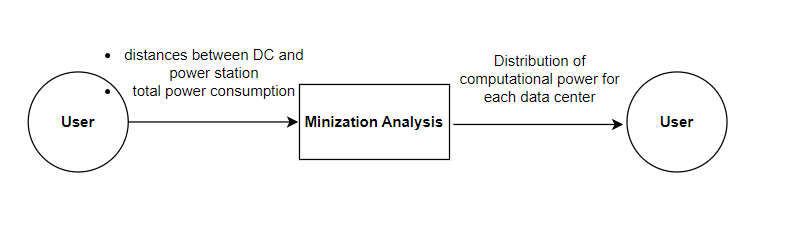
\includegraphics[width=0.6\textwidth]{system context Figure.png}
\caption{System Context}
\label{Fig_SystemContext} 
\end{center}
\end{figure}



\begin{itemize}
\item User Responsibilities:
\begin{itemize}
\item keep the unit even, keep every input with SI standard
\item Provide the distances between the power station and data centers and keep input under constraint.
\item Change system setting with their unique situations included total power consumption, renewable power rate and grid power rate.

\end{itemize}
\item \progname{Minimization Analysis} Responsibilities:
\begin{itemize}
\item Keep positive input and less than max limit
\item Detect if the output is capable for a data center to carry
\item Detect data type mismatch, such as relocate data under same unit
\end{itemize}
\end{itemize}

\subsection{User Characteristics} \label{SecUserCharacteristics}

{The front user should keep the unit with SI standard. The end user should have basic knowledge of undergraduate math and physics.}

\subsection{System Constraints}

\begin{itemize}
\item Grid Power Consumption Constraint: The grid power consumption for each data center should be within the user-defined maximum grid power consumption restriction.
\item Renewable Energy Constraint: The renewable energy consumption for each data center should not exceed the user-defined renewable energy limit.
\item Total Power Consumption Constraint: The sum of renewable energy and grid energy consumption for all data centers should be equal to the user-defined total power consumption.
\item Maximum Power Consumption per Data Center Constraint: The sum of renewable and grid energy consumption for each data center should not exceed the user-defined maximum power consumption per data center.
\item Power Loss Constraint: The power loss due to transmission lines (TL) should be accounted for when calculating the actual grid energy consumption for each data center.
\end{itemize}

\section{Specific System Description}

This section first presents the problem description, which gives a high-level
view of the problem to be solved.  This is followed by the solution characteristics
specification, which presents the assumptions, theories, definitions and finally
the instance models.

\subsection{Problem Description} \label{Sec_pd}

\progname{This model is intended to estimate the minimum cost with different computing distributions of data centers with different distances from electricity power station} \\

\subsubsection{Terminology and  Definitions}\label{ssc:terminology-definitions}
\label{ssc:TM}

 {The minimization problem involves finding the lowest possible value of an objective function while taking into account the constraints imposed on the problem. The ideal value is the minimum value of the objective function, which lies within the feasible region defined by the problem's restrictions. To better understand the problem, one can construct a graph representing the feasible region, which visually displays the viable combinations of variables. By examining this feasible region, it is possible to determine the optimized distribution of computing resources that adheres to the given constraints. }




\subsubsection{Physical System Description} \label{sec_phySystDescrip}

{Physics system will regarding to real world. HVDC transmission losses are quoted as less than 3\% per 1,000 km\textsuperscript{\cite{rosellon2003different}}, a formula was designed to calculate the total power lose along the transmission line. With various of distance as input, the system operation like a net flowing. Each data center will consuming electricity from both renewable resources and grid power station. In the model, only transmission along electricity grid will assume have power lose, renewable resource stations are assuming very close to the data centers the supplied.  }

The physical system of \progname{}, as shown in Figure2,
includes the following elements:

\begin{itemize}

\item Data centers are not uniformed in the area.

\item Renewable resources stations are very close to the data centers they supplied.

\end{itemize}
\begin{figure}[h!]
\begin{center}
 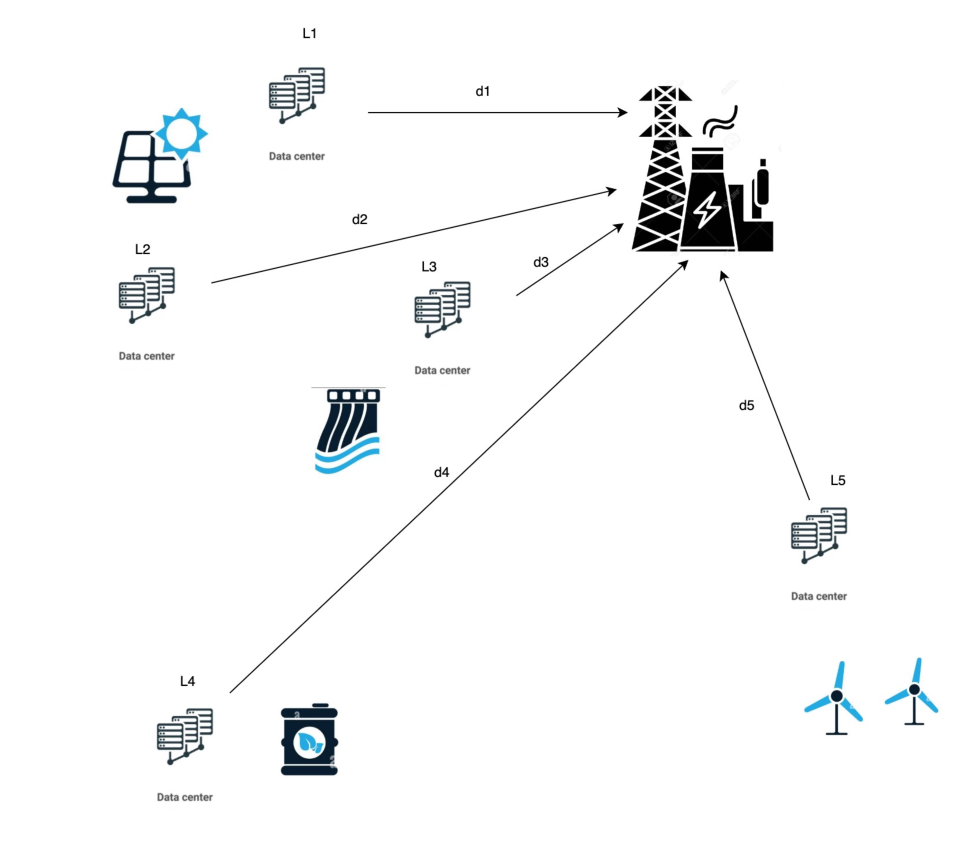
\includegraphics[width=0.6\textwidth]{distributed model.pdf}
\caption{System Context}
\label{Fig_SystemContext} 
\end{center}
\end{figure}


\subsubsection{Goal Statements}


\begin{itemize}

\item[GS\refstepcounter{goalnum}\thegoalnum \label{G_meaningfulLabel}:] {Develop a program that optimizes the power consumption and associated costs for a given set of data centers, taking into consideration their distances, rates of renewable and grid energy, and power consumption limits.}
\item[GS\refstepcounter{goalnum}\thegoalnum \label{G_meaningfulLabel}:] { Ensure that the program is user-friendly by prompting the user to input a CSV file containing relevant data, along with any specific grid power restrictions and renewable power limits.}
\item[GS\refstepcounter{goalnum}\thegoalnum \label{G_meaningfulLabel}:] {Design the program to be robust and flexible, able to handle cases where specific information is not provided by the user, by assigning default values when necessary.}
\item[GS\refstepcounter{goalnum}\thegoalnum \label{G_meaningfulLabel}:] { Provide clear, informative results that display the optimal power consumption for each data center, detailing the amounts of renewable and grid energy used, as well as the total cost, allowing users to make informed decisions regarding their data centers' energy consumption.}
\end{itemize}

\subsection{Solution Characteristics Specification}

 {This section characterizes the attributes of an acceptable solution. Both analysts and stakeholders should agree on these attributes so that the solution can be accepted when the project is complete.}


\subsubsection{Assumptions} \label{sec_assumpt}


This section simplifies the original problem and helps in developing the
theoretical model by filling in the missing information for the physical
system. The numbers given in the square brackets refer to the theoretical model
[T], general definition [GD], data definition [DD], instance model [IM], or
likely change [LC], in which the respective assumption is used.
\begin{itemize}

\item[A\refstepcounter{assumpnum}\theassumpnum \label{as:n}:]
  We know that distances as input should be positive and a reasonable number.

\item[A\refstepcounter{assumpnum}\theassumpnum \label{as:approximate}:]
  The software will estimate the distribution of load from a given total load. 


\item[A\refstepcounter{assumpnum}\theassumpnum \label{as:sixterm}:]
  The objective of setting power loss with a constant coefficient is to eliminate the impact of power loss in substations.
\item[A\refstepcounter{assumpnum}\theassumpnum \label{A_meaningfulLabel}:]
  {Depends on the pricing with $C_r$ and $C_p$,  the $L_i$ will be distributed with either descending or ascending order of di }

\end{itemize}

\subsubsection{Theoretical Models}\label{TM-series-cauchy-condition}
Applying the terminology and definitions from 4.1.1, this section records
theorems required to identify a minimum optimal solution.

Consider the total cost for all data centers this is the sum of the total grid power supply cost plus the total renewable supply cost. The computing power distribution will as the same proportion as their electricity consumption\textsuperscript{\cite{sedano2004electricity}}.
~\newline

\noindent
\deftheory
% #2 refname of theory
{T1}
% #3 label
{Minimize the cost}
% #4 equation
{ $C_\text {total}$=\sum_{i=1}^{n} $C_ri$ * $R_i$+$C_pi$ * $P_i$}
% #5 description
{
  The above equation gives the value of the total cost for given Cr and Cp with power consumption as Ri and Pi respectively.
  When solving a minimizing problem, some constrain of variables must apply to find the feasible region. 
}
% #6 Notes
{
None.
}
% #7 Source
{
  \url{https://www.superprof.co.uk/resources/academic/maths/linear-algebra/linear-programming/steps-to-solve-a-linear-programming-problem.html}
}
% #8 Referenced by
{
  GD2
}
% #9 Preconditions
{
None
}
% #1 derivation - not applicable by default
{}
\noindent
\deftheory
% #2 refname of theory
{T2}
% #3 label
{Calculate for $P_i$}
% #4 equation
{
  \mathrm{$P_i$}=\mathrm{$P_\text{i-theoretical}$} *(1-(0.03 \mathrm{$d_i$} / 1000)) 
}
% #5 description
{
  The above equation gives the value of power lose with transmission distance varied. The Pi is the actual consumption of energy, Pi-theoretical is the consumption without transmission lose. HVDC transmission losses are quoted as less than 3\% per 1,000 km 
}
% #6 Notes
{
None.
}
% #7 Source
{
 See Reference
}
% #8 Referenced by
{
  GD1
}
% #9 Preconditions
{
None
}
\noindent
\deftheory
% #2 refname of theory
{T3}
% #3 label
{The power consumption for each data center}
% #4 equation
{
  $L_\text {total}$=\sum_{i=1}^{n} $L_i$ = $R_i$ + $P_i$
}
% #5 description
{
  The power consumption for each data center will come up with renewable supply and grid power supply. 
}
% #6 Notes
{
None.
}
% #7 Source
{
  See Reference
}
% #8 Referenced by
{
 GD1
}
% #9 Preconditions
{
None
}

~\newline

\subsubsection{General Definitions}\label{sec_gendef}

General Definitions (GDs) are a refinement of one or more TMs, and/or of
  other GDs.  The GDs are less abstract than the TMs.  Generally the reduction
  in abstraction is possible through invoking referencing Assumptions. This section collects the laws and equations that will be used in building the
instance models.

~\newline

\noindent
\begin{minipage}{\textwidth}
\renewcommand*{\arraystretch}{1.5}
\begin{tabular}{| p{\colAwidth} | p{\colBwidth}|}
\hline
\rowcolor[gray]{0.9}
Number& GD\refstepcounter{defnum}\thedefnum \label{NL}\\
\hline
Label &\bf Power losses along transmission line \\
\hline
% Units&$MLt^{-3}T^0$\\
% \hline
SI Units&\si{\kWh}\\
\hline
Equation& Loss= 0.03 * $d_i$/1000 \\
\hline
Description &  
                Transmission and distribution (T\&D) loss are amounts that are not paid for by users.

\\

\\
\hline
  Source & \url{https://www.electricalindia.in/losses-in-distribution-transmission-lines/#:~:text=Transmission%20and%20distribution%20(T%26D,))%20%2F%20Energy%20Input%20kwh%20x100.} \\
  \hline
  Ref.\ By & T2\\
  \hline
\end{tabular}
\end{minipage}\\

\subsubsection*{Detailed derivation of calculating power transmission losses}

{It is fact that the unit of electric energy generated by the power station does not match the units distributed to the consumers. Some percentage of the units is lost in the distribution network. This difference in the generated \& distributed units is known as transmission and distribution losses. Distribution Sector is considered the weakest link in the entire power sector. Transmission losses are approximately 17\% while distribution losses are approximately 50\%. In this model, we assume all of the data centers pass through the same number of sectors, so only transmission line losses are calculated.}

\subsubsection{Data Definitions}\label{sec_datadef}

{The Data Definitions are definitions of symbols and equations that are
  given for the problem.  They are not derived; they are simply used by other
  models.  For instance, if a problem depends on density, there may be a data
  definition for the equation defining density.  The DDs are given information
  that you can use in your other modules.}

{All Data Definitions should be used (referenced) by at least one other
  model.}

This section collects and defines all the data needed to build the instance
models. The dimension of each quantity is also given.  {Modify the examples
  below for your problem, and add additional definitions as appropriate.}

~\newline

\noindent
\begin{minipage}{\textwidth}
\renewcommand*{\arraystretch}{1.5}
\begin{tabular}{| p{\colAwidth} | p{\colBwidth}|}
\hline
\rowcolor[gray]{0.9}
Number& DD\refstepcounter{datadefnum}\thedatadefnum \label{FluxCoil}\\
\hline
Label& \bf Level of load (computing power) for each data center\\
\hline
Symbol &$L_p$\\
\hline
% Units& $Mt^{-3}$\\
% \hline
  SI Units & \si{MW}\\
  \hline
  Equation& None\\
  \hline
  Description & 
               In each data center, the load represents its computational power. This means that a higher load indicates a greater capacity to process and handle complex tasks and large amounts of data. As the load increases, the data center can effectively manage more simultaneous operations, ensuring efficient performance and meeting the demanding needs of today's data-driven world.
  \\
  \hline
  Sources& \url{https://bitflyer.com/en-eu/s/glossary/hashrate}\\
  \hline
  Ref.\ By & \iref{ewat}\\
  \hline
\end{tabular}
\end{minipage}\\


\subsubsection{Instance Models} \label{sec_instance}    

{The motivation for this section is to reduce the problem defined in
  ``Physical System Description'' (Section~\ref{sec_phySystDescrip}) to one
  expressed in mathematical terms. The IMs are built by refining the TMs and/or
  GDs.  This section should remain abstract.  The SRS should specify the
  requirements without considering the implementation.}

This section transforms the problem defined in Section~\ref{Sec_pd} into 
one which is expressed in mathematical terms. It uses concrete symbols defined 
in Section~\ref{sec_datadef} to replace the abstract symbols in the models 
identified in Sections~\ref{sec_gendef}.

The goals {reference your goals} are solved by {reference your instance
  models}.  {other details, with cross-references where appropriate.}
{Modify the examples below for your problem and add additional models as
  appropriate.}

~\newline

%Instance Model 1

%~\newline


\subsubsection{Input Data Constraints} \label{sec_DataConstraints}    

Table~\ref{TblInputVar} shows the data constraints on the input output
variables.  The column for physical constraints gives the physical limitations
on the range of values that can be taken by the variable.  The column for
software constraints restricts the range of inputs to reasonable values.  The
software constraints will be helpful in the design stage for picking suitable
algorithms.  The constraints are conservative, to give the user of the model the
flexibility to experiment with unusual situations.  The column of typical values
is intended to provide a feel for a common scenario.  The uncertainty column
provides an estimate of the confidence with which the physical quantities can be
measured.  This information would be part of the input if one were performing an
uncertainty quantification exercise.

The specification parameters in Table~\ref{TblInputVar} are listed in
Table~\ref{TblSpecParams}.

\begin{table}[!h]
  \caption{Input Variables} \label{TblInputVar}
  \renewcommand{\arraystretch}{1.2}
\noindent \begin{longtable*}{l l l l c} 
  \toprule
  \textbf{Var} & \textbf{Physical Constraints} & \textbf{Software Constraints} &
                             \textbf{Typical Value} & \textbf{Uncertainty}\\
  \midrule 
  $di$ & $di > 0$ & 0 \leq di \leq $d_{\text{max}}$ & 1000 \si[per-mode=symbol] {\metre} & 10\%
  \\
  $L_\text{total}$ & $L_\text{total}$ $> 0$ & 0 \leq $L_\text{total}$ \leq $L_{\text{max}}$ & 10 MWh & 10\%
  \\
  \bottomrule
\end{longtable*}
\end{table}

\noindent 
\begin{description}
\item[(*)] {the system able to convert MWh to KWh}
\end{description}

\begin{table}[!h]
\caption{Specification Parameter Values} \label{TblSpecParams}
\renewcommand{\arraystretch}{1.2}
\noindent \begin{longtable*}{l l} 
  \toprule
  \textbf{Var} & \textbf{Value} \\
  \midrule 
  $C_r$ & 0 $< $C_\text{ri}$ $< $L_\text{max}$\\
  $C_p$ & 0 $< $C_\text{pi}$ $< $L_\text{max}$\\
  \bottomrule
\end{longtable*}
\end{table}

\subsubsection{Properties of a Correct Solution} \label{sec_CorrectSolution}

\noindent
A correct solution must exhibit {fill in the details}.  {These
  properties are in addition to the stated requirements.  There is no need to
  repeat the requirements here.  These additional properties may not exist for
  every problem.  Examples include conservation laws (like conservation of
  energy or mass) and known constraints on outputs, which are usually summarized
  in tabular form.  A sample table is shown in Table~\ref{TblOutputVar}}

\begin{table}[!h]
\caption{Output Variables} \label{TblOutputVar}
\renewcommand{\arraystretch}{1.2}
\noindent \begin{longtable*}{l l} 
  \toprule
  \textbf{Var} & \textbf{Physical Constraints} \\
  \midrule 
  $A_i$ & Under data center computational power capable size
  \\
  \bottomrule
\end{longtable*}
\end{table}


\section{Requirements}

{The requirements refine the goal statement.  They will make heavy use of
  references to the instance models.}

This section provides the functional requirements, the business tasks that the
software is expected to complete, and the nonfunctional requirements, the
qualities that the software is expected to exhibit.

\subsection{Functional Requirements}

\noindent \begin{itemize}

\item[R\refstepcounter{reqnum}\thereqnum \label{R_Inputs}:] {The system shall allow the user to input a CSV file containing information on data centers and their power consumption, renewable energy rate, and grid energy rate.}

\item[R\refstepcounter{reqnum}\thereqnum \label{R_OutputInputs}:] {The system shall extract and display the number of data centers, their distances, the rate of renewable energy, the rate of grid energy, the total power consumption, and the maximum power consumption per data center from the CSV file.}

\item[R\refstepcounter{reqnum}\thereqnum \label{R_Calculate}:] {User should keep input validate data type and reasonable value.}

\item[R\refstepcounter{reqnum}\thereqnum \label{R_VerifyOutput}:]
  {The system shall solve the optimization problem using linear programming to calculate the optimal power consumption for each data center.}

\item[R\refstepcounter{reqnum}\thereqnum \label{R_Output}:] {The system shall display the optimal power consumption for each data center, including the amount of renewable energy and grid energy used.}
\item[R\refstepcounter{reqnum}\thereqnum \label{R_VerifyOutput}:]
  {The system shall calculate the total cost of the optimal power consumption.}
  \item[R\refstepcounter{reqnum}\thereqnum \label{R_VerifyOutput}:]
  {The system shall plot a graph of the optimal power consumption for each data center against their distances, with the y-axis representing the total power consumption.}
\end{itemize}


\subsection{Nonfunctional Requirements}


\noindent \begin{itemize}

\item[NFR\refstepcounter{nfrnum}\thenfrnum \label{NFR_Accuracy}:]
  \textbf{Accuracy} {The computed solutions must meet the accuracy level required for engineering applications.}

\item[NFR\refstepcounter{nfrnum}\thenfrnum \label{NFR_Usability}:] \textbf{Usability}
  {The program should not have a user interface, but the output should be easy to read and copy.}

\item[NFR\refstepcounter{nfrnum}\thenfrnum \label{NFR_Maintainability}:]
  \textbf{Maintainability} { The time complexity of the program must be O(n) to ensure maintainability.}

\item[NFR\refstepcounter{nfrnum}\thenfrnum \label{NFR_Portability}:]
  \textbf{Portability} {The program must be easily integrable with other software programs.}


\end{itemize}

\section{Likely Changes}    

\noindent \begin{itemize}

\item[LC\refstepcounter{lcnum}\thelcnum\label{LC_meaningfulLabel}:] { It is likely that the program will need to include additional options for renewable energy supply.}
\item[LC\refstepcounter{lcnum}\thelcnum\label{LC_meaningfulLabel}:] {The program may be modified to perform process analysis under minimum CO2 emissions in addition to operating the analysis under minimum cost.}
\item[LC\refstepcounter{lcnum}\thelcnum\label{LC_meaningfulLabel}:] { It is probable that the program will need to be made more flexible to accommodate a wider range of operating systems.}
\end{itemize}

\section{Unlikely Changes}    

\noindent \begin{itemize}

\item[ULC 1\label{LC_meaningfulLabel}]:{The basic design concept of allocate computing instead of power station will unlikely to change.}

\end{itemize}
\section{Traceability Matrices and Graphs}

{The purpose of the traceability matrices is to provide easy references on what
has to be additionally modified if a certain component is changed.  Every time a
component is changed, the items in the column of that component that are marked with an ``X'' may have to be modified as well.  Table~\ref{Table:trace} shows the
dependencies of theoretical models, general definitions, data definitions, and instance models with each other.  Table~\ref{Table:R_trace} shows the dependencies of theoretical models,
general definitions, data definitions, instance models, and likely changes on the assumptions.}


\begin{table}[h!]
    \centering
    \begin{tabular}{|l|l|l|l|l|l|l|}
    \hline
        ~ & T1 & T2 & T3 & GD1 & DD1 & IM1 \\ \hline
        T1 & ~ & x & x & ~ & ~ & ~ \\ \hline
        T2 & ~ & ~ & ~ & ~ & x & ~ \\ \hline
        T3 & ~ & ~ & ~ & ~ & x & ~ \\ \hline
        GD1 & ~ & x & ~ & ~ & ~ & ~ \\ \hline
        DD1 & ~ & ~ & x & ~ & ~ & ~ \\ \hline
        IM1 & ~ & ~ & x & ~ & ~ & ~ \\ \hline
    \end{tabular}

\caption{Traceability Matrix Showing the Connections Between Items of Different Sections}
\label{Table:trace}
\end{table}

\begin{table}[!ht]
    \centering
    \begin{tabular}{|l|l|l|l|l|l|}
    \hline
        ~ & A1 & A2 & A3 & A4 & A5 \\ \hline
        T1 & ~ & ~ & ~ & ~ & ~ \\ \hline
        T2 & x & ~ & x & ~ & ~ \\ \hline
        T3 & ~ & ~ & ~ & x & x \\ \hline
        GD1 & ~ & x & ~ & ~ & ~ \\ \hline
        DD1 & ~ & x & ~ & ~ & ~ \\ \hline
        IM1 & ~ & ~ & ~ & ~ & ~ \\ \hline
    \end{tabular}
\caption{Traceability Matrix Showing the Connections Between Assumptions}
\label{Table:R_trace}
\end{table}

\section{Values of Auxiliary Constants}
Grid Power restrictions:
\begin{equation}
\mathrm{Grid\textunderscore Power\textunderscore restrictions}
\end{equation}

Renewable limits:
\begin{equation}
\mathrm{Renewable\textunderscore limits}
\end{equation}

Rate of renewable energy :
\begin{equation}
\mathrm{rate\textunderscore renewable}
\end{equation}

Rate of grid energy :
\begin{equation}
\mathrm{rate\textunderscore grid}
\end{equation}

Maximum power consumption per data center:
\begin{equation}
\mathrm{max\textunderscore power\textunderscore consumption}
\end{equation}


\bibliographystyle {unsrt}
\bibliography{references}

\end{document}